\documentclass[border=2pt]{standalone}
\usepackage{tikz}
\usetikzlibrary{trees}
\begin{document}
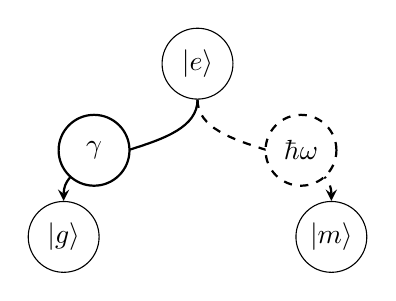
\begin{tikzpicture}[
  grow=down,
  level distance=22mm,
  sibling distance=34mm,
  every node/.style={draw,circle,minimum size=9mm,inner sep=1pt},
  edge from parent/.style={draw,thick,-stealth},
  edge from parent path={
    (\tikzparentnode.south) .. controls +(0,-7mm) and +(0,7mm) .. (\tikzchildnode.north)
  }
]
  \node {$|e\rangle$}
    child {
      node {$|g\rangle$}
      edge from parent node[left,fill=white,inner sep=1pt] {$\gamma$}
    }
    child {
      node {$|m\rangle$}
      edge from parent[dashed]
        node[right,fill=white,inner sep=1pt] {$\hbar\omega$}
    };
\end{tikzpicture}
\end{document}
